\subsection{The set of fragments}

A pangenome fragment can come from:

\begin{enumerate}
  \item a unique contig of \(Asm_1\)

  \item a unique contig of \(Asm_2\)

  \item at least one contig of \(Asm_1\) and at least one contig of \(Asm_2\)
\end{enumerate}

\begin{missingproofbox}
  There is no share such that all its contigs come from the same assembler
\end{missingproofbox}

In cases 1 and 2, the fragment is defined as a \emph{subcontig}, while in case 3 it is defined as a shared subcontig (\emph{a share}).

For a fragment \(i \in \Fragments{}\), \(\Contigs{}(i) \subset \Contigs{}\) denotes the set of contigs from which \(i\) comes from. The fragment \(i\) is a subcontig if and only if \(|\Contigs{}(i)| = 1\), otherwise \(i\) is a share if and only if \(|\Contigs{}(i)| > 1\).
The extremity vertices in \(V\) of a fragment \(i \in \Fragments{}\) are provided by \(i_t \in V_t\) and \(i_h \in V_h\) (note that \(\Set{i_t, i_h} \in \EFrags{}\)). Reversely, \(vfrag \colon V \tosur \Fragments{}\) gives the fragment associated to one of its extremity vertices.

\subsubsection{Fragment properties}

Each fragment is associated with three properties: its coverage, its plasmidness and a set of GC penalties depending on GC content intervals.

\begin{definition}{Fragment coverage}{fragment_coverage}
  \begin{todobox}
    Explain why we do not normalize as Cédric Chauve proposed.
  \end{todobox}
  Let \(i \in \Fragments{}\) be a fragment.
  By \(\cov{i} \in \Reals{}_{>0}\) we denote its coverage:
  \[
    \cov{i} = \max_{c \in \Contigs{}(i)}\Set*{\cov{c}}
  \]
\end{definition}

\begin{newfeatbox}
  While PlasBin-flow uses a GC content penalty, we use a GC probability score

  \begin{questionbox}
    Before we had a penalty.
    The flow can pass through loops and cycles, without changing the total flow (because of the conservation constraints). But the GC content penalties prevent us to use more fragments otherwise the objective value is most likely to decrease.

    That can explain why some bins are split into several bins.
  \end{questionbox}

  \begin{questionbox}
    I the one hand, computing the fragment GC penalties from the contigs, and correct the penalties for the share, favours to keep the original contigs.

    Computing the fragment GC penalties from the contigs means we trust the contig assemblies (as in the formula, the length parameter is the length of the contig, not these of its fragments)

    In the other hand, recomputing the fragment GC penalties and thus using as the length parameter the length of the fragment may result in a strong statistical bias for short fragments.

    \begin{notebox}
      Here we chose to recompute the GC probabilities without taking into account from which contigs a fragment belongs.
    \end{notebox}
  \end{questionbox}
\end{newfeatbox}

\begin{definition}{Fragment GC probability score}{fragment_GC_score}
  Let \(i \in \Fragments{}\) be a contig and \(b\) be a GC content interval.
  By \(\gcscore{i}{b} \in [-1, 1]\) we denote the GC probability score of the fragment \(i\) according to the GC content interval \(b\):
  \[
    \gcscore{i}{b} = 2 \frac{\Pr(n|b,l)\Pr(b)}{\max\limits_{b' \in K}\Set*{\Pr(n|b',l)\Pr(b')}} - 1
  \]
  Where \(K\) is the set of GC content intervals, \(n\) is the number of GC in the fragment of length \(l\), and \(\Pr(n|b,l)\) is calculated as described in~\cite{manePlasBinflowFlowbasedMILP2023}, Section 2.5.1.

  \begin{fixmebox}
    Adapt the correction constraints according to the new score definition.
  \end{fixmebox}
\end{definition}

\begin{definition}{Fragment gene density}{frag_gene_density}
  \begin{newfeatbox}
    We recompute the gene density of the fragments according to the position of the fragments on the contigs.
  \end{newfeatbox}

  \begin{refactorbox}
    Generalize gene density to plasmidness score
  \end{refactorbox}
  Let \(i\) be a pangenome fragment.
  By \(\gd{i} \in [0, 1]\) we denote its gene density:
  \[
    \gd{i} = \frac{1}{ |i| \times |\Contigs{}(i)| } \sum_{\substack{
        c \in \Contigs{}(i) \\
    }} \ncovnuc{c}(\fcstart{i}{c}, \fcend{i}{c})
  \]
  Where \(\ncovnuc{c}(\fcstart{i}{c}, \fcend{i}{c})\) is the number of nucleotides of contig \(c\) covered by gene mapping matches between positions defined by \(i\) on \(c\).
\end{definition}

\subsubsection{Seed fragment candidates}

\begin{notebox}
  A first solution can be using the same computation as in PlasBin-flow, however, a gene can be contained in a contig, while a gene can correspond to a sequence of fragments.
\end{notebox}

We map genes from a plasmid gene reference database to the contigs.
As in~\cite{manePlasBinflowFlowbasedMILP2023}, we determine a pair of thresholds \((l, gd)\) maximizing the expression \(SP - NPS\) (see the description in the paper).
However, as the length and the gene density distributions differ between the assembled reference read dataset and the pangenome fragments, we normalize each threshold according to the distributions difference (according to the medians \(m\) and \(m'\)):

\[
  (l', gd') = \parenth*{\frac{m'}{m} l, \frac{m'}{m} gd}
\]

Thus, a fragment \(i \in \Fragments{}\) is in the seed fragment set \SeedFrags{} if, and only if \(|i| \geq l'\) and \(\gd{i} \geq gd'\).

\begin{newfeatbox}
  Here we take care of normalizing according the distribution of the parameters we filter (not done in PlasBin-flow)
\end{newfeatbox}

\Cref{fig:seed_frag-split_plasmid_gene} can help to find a seed definition and constraints adapted to fragments in the pan-assembly graph.

\begin{figure}[htb]
  \centering
  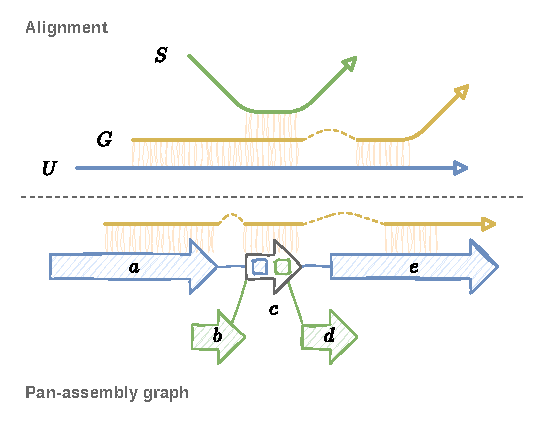
\includegraphics[width=0.6\linewidth]{pan-assembly_graph/img/seed_fragments-split_plasmid_gene.pdf}
  \figurecaption{The effect of fragmentation on plasmid gene mapping.}{%
    The top figure part represents a plasmid gene \(G\) (in orange) that partially maps onto Unicycler contig \(U\) (in blue) and SKESA contig \(S\) (in green).
    The bottom part illustrates the resulting pan-assembly subgraph, where fragments \(a\), \(c\) and \(e\) are defining contig \(U\), while fragments \(b\), \(c\), \(d\) are defining contig \(S\).
  }\label{fig:seed_frag-split_plasmid_gene}
\end{figure}